\documentclass[10pt]{article}
% Эта строка — комментарий, она не будет показана в выходном файле
\usepackage{ucs}
\usepackage[utf8x]{inputenc} % Включаем поддержку UTF8
\usepackage[russian]{babel}  % Включаем пакет для поддержки русского языка
\usepackage{amsmath}
\usepackage{amssymb}
\usepackage{mathtools}

\hoffset=0mm
\voffset=0mm
\textwidth=170mm        % ширина текста
\oddsidemargin=-0mm   % левое поле 25.4 - 5.4 = 20 мм
\textheight=240mm       % высота текста 297 (A4) - 40
\topmargin=-15.4mm      % верхнее поле (10мм)
\headheight=5mm      % место для колонтитула
\headsep=5mm          % отступ после колонтитула
\footskip=8mm         % отступ до нижнего колонтитула



% \textwidth=180mm    
% \oddsidemargin=-10mm 

\title{Лабораторная работа № 2.2: {\it Изучение затухающих колебаний в колебательном контуре.}}
\author{Зотов Алексей, 497}
\date{\today}

\begin{document}

\maketitle
\textbf{Цель работы:} Изучение параметров и характеристик колебательного контура.

\textbf{В работе испольуются:} \small{генератор звуковых сигналов, осциллограф, модуль с колебательным контуром ФПЭ–10, преобразователь импульсов ФПЭ–08, источник питания, магазин сопротивлений.}

\textbf{Ход работы:}
    \begin{enumerate}
    \item \textbf{Измерение периода, логарифмического декремента и параметров колебательного контура.} \\
    $l_1 = 3.8 $ см, $l = 0.7$ см, $\nu = 250$ Гц \\
    \begin{equation}
        T = \frac{l}{l_1 \nu} \approx 7.37 \cdot 10^{-3} \text{с} 
    \end{equation}
    Замерим последовательные амплитуды и найдем $\lambda = \ln{\frac{U_n}{U_{n+1}}}$ , $\gamma = \lambda/T$\\

    $R = 100 $ [Ом] \\ 
    $U_{A} = [3.8,1.3,0.8,0.6,0.4]$ [В] \\
    $\lambda = [1.1, 0.5, 0.3, 0.4] $ \\ 
    $\lambda_{\text{ср.}} = 0.56$ \\ 
    $\gamma = 764 [c^{-1}]$ \\ 
    \\
    $R = 200 $ [Ом] \\ 
    $U_{A} = [3.4,1.0,0.5,0.3,0.2]$ [В] \\
    $\lambda = [1.2, 0.7, 0.5, 0.4] $ \\ 
    $\lambda_{\text{ср.}} = 0.71$ \\ 
    $\gamma = 961 [c^{-1}]$ \\ 
    \\
    $R = 300 $ [Ом] \\ 
    $U_{A} = [5.8,1.4,0.5,0.2]$ [В] \\
    $\lambda = [1.4, 1.0, 0.9] $ \\ 
    $\lambda_{\text{ср.}} = 1.1$ \\ 
    $\gamma = 1523 [c^{-1}]$ \\ 
    \\
    $R = 400 $ [Ом] \\ 
    $U_{A} = [5.2,1.0,0.25]$ [В] \\
    $\lambda = [1.6, 1.4] $ \\ 
    $\lambda_{\text{ср.}} = 1.5$ \\ 
    $\gamma = 2059 [c^{-1}]$ \\ 
    \\
    $R = 500 $ [Ом] \\ 
    $U_{A} = [4.6,0.7,0.1]$ [В] \\
    $\lambda = [1.9, 1.9] $ \\ 
    $\lambda_{\text{ср.}} = 1.9$ \\ 
    $\gamma = 2598 [c^{-1}]$ \\ 
    \\
    $R = 600 $ [Ом] \\ 
    $U_{A} = [4.2,0.5]$ [В] \\
    $\lambda = 2.12 $ \\ 
    $\gamma = 2888 [c^{-1}]$ \\ 
    Приблизим зависимость $\lambda(R_m)$ прямой $a R_m + b$ с помощью МНК, тогда : 
    \begin{equation}
        \lambda = \frac{R}{2 L} T = \frac{T}{2 L} (R_m + R_k) \implies L = \frac{T}{2 a}
    \end{equation}

    \begin{equation}
        R_k = \frac{2 b L}{T}
    \end{equation}

    \begin{center}
    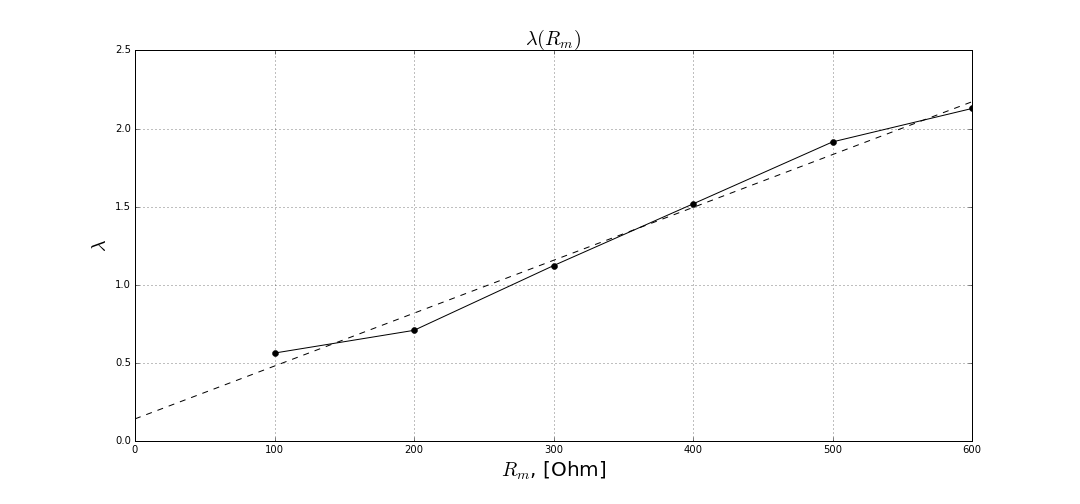
\includegraphics[width=14cm,height=6cm]{plot1.png}
    \end{center}
    $a = (3.38 \pm 0.16) * 10^{-3} $, $b = (0.14 \pm 0.03)$ \\ 
    $L = 0.109 \pm 0.005$ [Гн] , $ R_k = 42 \pm 9$ [Ом]. \\ \\
    \begin{equation}
        Q = \frac{\pi}{\gamma T} = \frac{1}{R}\sqrt{\frac{L}{C}} \implies C = \frac{L \gamma^2 T^2}{\pi^2 (R_k + R_m)^2}
    \end{equation}
    \begin{equation}
        \varepsilon^2_C \approx \varepsilon^2_L + \varepsilon^2_{R_k} 
    \end{equation}
    $C = [ 1.74 , 0.95 , 1.19 , 1.30, 1.38 ,1.21] \cdot 10^{-7}$ [Ф]. \\
    $C_{\text{ср}} = (1.29 \pm 0.11 )\cdot 10^{-7}$ [Ф]. \\ 
    $\varepsilon_{C_{cp}} \approx 8.7 \%$\\
    $R_{mkr} = 2 \sqrt{\frac{L}{C]}} - R_k \approx 1793$ [Ом].\\

    \item \textbf{Исследование фазовых кривых.} \\
    



    \end{enumerate}
\end{document}